\begin{frame}{Applikation}
	\begin{center}
		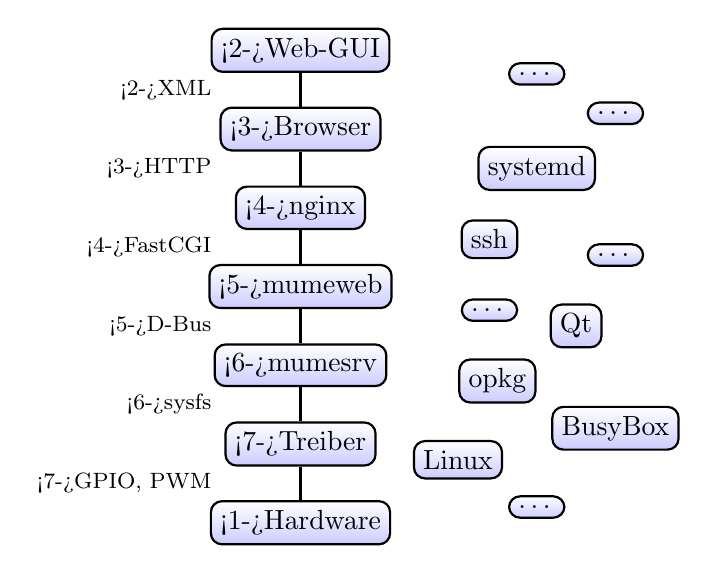
\begin{tikzpicture}[thick]
			\tikzstyle{every node}=[shape=rectangle, rounded corners,
				draw, align=center, top color=white, bottom color=blue!20]
			\node at (0,0) (hw) {{\visible<1->{Hardware}}};
			\node at (0,1) (driver) {{\visible<7->{Treiber}}};
			\node at (0,2) (srv) {{\visible<6->{mumesrv}}};
			\node at (0,3) (web) {{\visible<5->{mumeweb}}};
			\node at (0,4) (server) {{\visible<4->{nginx}}};
			\node at (0,5) (browser) {{\visible<3->{Browser}}};
			\node at (0,6) (gui) {{\visible<2->{Web-GUI}}};
			
			\visible<8-> {
				\node at (2,0.8) {Linux};
				\node at (4,1.2) {BusyBox};
				\node at (2.5,1.8) {opkg};
				\node at (3.5,2.5) {Qt};
				\node at (2.4,3.6) {ssh};
				\node at (3,4.5) {systemd};
			}
			
			\visible<9-> {
				\node at (2.4,2.7) {\ldots};
				\node at (3,0.2) {\ldots};
				\node at (4,3.4) {\ldots};
				\node at (4,5.2) {\ldots};
				\node at (3,5.7) {\ldots};
			}
			
			\tikzstyle{every node}=[midway,left=10mm,font=\footnotesize]
			\draw (hw) -- (driver) node {{\visible<7->{GPIO, PWM}}};
			\draw (driver) -- (srv) node {{\visible<6->{sysfs}}};
			\draw (srv) -- (web) node {{\visible<5->{D-Bus}}};
			\draw (web) -- (server) node {{\visible<4->{FastCGI}}};
			\draw (server) -- (browser) node {{\visible<3->{HTTP}}};
			\draw (browser) -- (gui) node {{\visible<2->{XML}}};
		\end{tikzpicture}
	\end{center}
\end{frame}

\begin{frame}{Hardware}
	\begin{multicols}{2}
		Add picture of mume device
		\begin{center}
			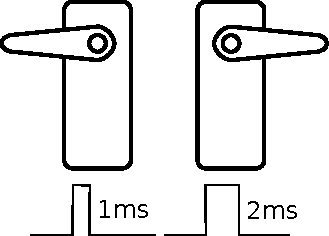
\includegraphics[width=4cm]{res/servo_pwm.pdf}
		\end{center}
	\end{multicols}
\end{frame}

\begin{frame}[fragile]{mume Device Tree}
	\begin{multicols}{2}
		\begin{lstlisting}[frame=,numbers=none,language=]
mume {
  compatible = "urs,mume";
  status = "okay";

  gpio = <&gpio1 28 GPIO_ACTIVE_LOW>;
  pwms = <&ehrpwm1 0 10000000 0>;

  pinctrl-names = "default";
  pinctrl-0 = <&mume_pins>;
};

mume_pins: mume_pins {
  pinctrl-single,pins = <
    0x78 (MUX_MODE7 | PIN_INPUT_PULLUP)
    0x48 (MUX_MODE6 | PIN_OUTPUT)
  >;
};
		\end{lstlisting}
\pagebreak
		\begin{flushright}
		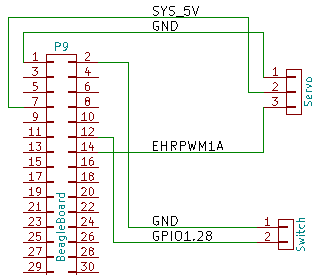
\includegraphics[width=4.3cm]{res/mume_schematic.pdf}
		\end{flushright}
	\end{multicols}
\end{frame}

\begin{frame}{Hardware ansteuern}
	\begin{multicols}{2}
		\begin{center}
			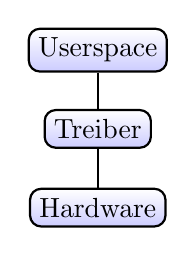
\begin{tikzpicture}[thick,
				every node/.style = {shape=rectangle, rounded corners,
					draw, align=center,
					top color=white, bottom color=blue!20}]]

				\node (userspace) {Userspace};
				\node[below of=userspace] (driver) {Treiber};
				\node[below of=driver] (hardware) {Hardware};
				
				\draw (userspace) to (driver);
				\draw (driver) to (hardware);
			\end{tikzpicture}
			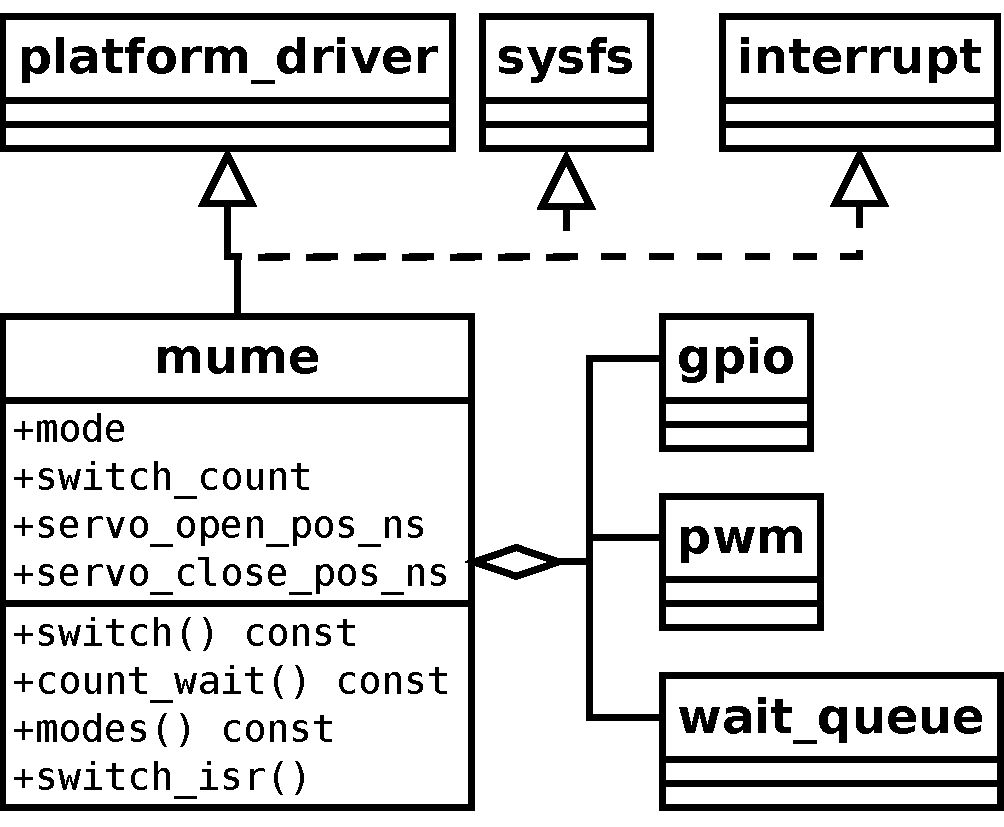
\includegraphics[width=0.5\textwidth]{res/mumedriver}
		\end{center}
	\end{multicols}
	\only<handout>{
		\begin{itemize}
			\item wie können wir die Hardware ansteuern?
			\item[$\rightarrow$] Linux Treiber, Frameworks, Infrastructure:
			\begin{itemize}
				\item Framework für Treiber
				\item Infrastrukur um auf Subsysteme zuzugreifen
			\end{itemize}
		\end{itemize}
	}
\end{frame}

\begin{frame}{vom Treiber zum Webserver}
	\begin{center}
		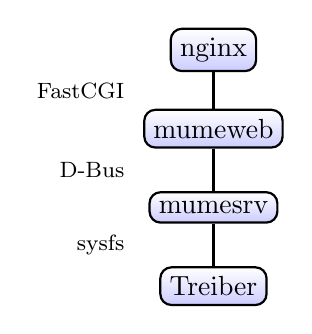
\begin{tikzpicture}[thick]
			\tikzstyle{every node}=[shape=rectangle, rounded corners,
				draw, align=center, top color=white, bottom color=blue!20]

			\node at (0,1) (driver) {Treiber};
			\node at (0,4) (server) {nginx};
			
			\visible<2->{
				\node at (0,2) (srv) {mumesrv};
			}
			
			\visible<3->{
				\node at (0,3) (web) {mumeweb};
			}

			\tikzstyle{every node}=[midway,left=10mm,font=\footnotesize]
			\visible<2->{
				\draw (driver) -- (srv) node {sysfs};
			}
			\visible<3->{
				\draw (web) -- (server) node {FastCGI};
			}
			\visible<4->{
				\draw (srv) -- (web) node {D-Bus};
			}
			
		\end{tikzpicture}
	\end{center}
\end{frame}
\note{
	\begin{itemize}
		\item mumeweb
		\begin{itemize}
			\item FastCGI / XML Interface
			\item (Session Handling)
		\end{itemize}
		\item mumesrv
		\begin{itemize}
			\item Persistenz
			\item D-Bus Interface
		\end{itemize}
	\end{itemize}
}

\begin{frame}{Service Manager}
	\begin{itemize}
		\item Wie starten und managen wir die Services?
		\item[$\rightarrow$] systemd
		\begin{itemize}
			\item service files schreiben
		\end{itemize}
	\end{itemize}
\end{frame}

\begin{frame}{Produktiv Image}
	\begin{itemize}
		\item Wie können wir die Firmware verteilen?
		\item[$\rightarrow$] Yocto
		\begin{itemize}
			\item Rezepte für Services
			\item anpassen bestehender Rezepte (nginx, qt, \ldots)
			\item Rezept für image
		\end{itemize}
		\item bitbake image
	\end{itemize}
\end{frame}

%\begin{frame}{Was passiert bei einem Tastendruck in der Web-Applikation}
%	Geht runter:
%	\begin{itemize}
%		\item SVG, Javascript
%		\item XML/HTTP
%		\item FastCGI
%		\item MumeWeb
%		\item D-Bus
%		\item MumeSrv
%		\item SysFS
%		\item Kernel
%		\item MUME-Treiber
%		\item PWM
%		\item Servo bewegt sich!
%	\end{itemize}
%\end{frame}
